\documentclass[12pt]{article}

\usepackage{graphicx}
\usepackage{graphicx}
\usepackage{caption}
\usepackage[spanish]{babel}
\usepackage[utf8]{inputenx}
\usepackage{anysize} 
\usepackage{amsmath}
\usepackage{listings}
\marginsize{2cm}{2cm}{1cm}{2cm} %izq der arriba abajo
\usepackage{hyperref}
\usepackage{wrapfig} % paquete gráfico

\hypersetup{
    colorlinks,%
    citecolor=black,%
    filecolor=black,%
    linkcolor=black,%
    urlcolor=black
}

\title{Informe Trabajo Profesional}
\author{Facundo Nahuel Uriel Silva, Estanislao López Morgan}

\begin{document}

  %Caratula
  \newpage
  \thispagestyle{empty}
  
  \begin{center}
    
\includegraphics[width=250px]{../logo_fiuba_alta.jpg} 

  \vspace{100px}

  \huge{Trabajo Profesional de Ingeniería Electrónica}
  \vspace{50px}

  \bf{ \huge{Sistema de control de fabricación de nano polvos mediante el proceso de sinterizado} }


  \vspace{80px}

  \end{center}
  
  \begin{bf}
    \begin{Large}
      \begin{tabbing}
	\= ----- \= ----- \= --------------------- \= \kill
	\> Integrantes:\\
	\\
	  \>\> Estanislao López Morgan \\
	  \>\>\>  Padrón:	\> 84546 \\
	  \>\>\>  Mail:	\>\url{estanux@gmail.com} \\
	\\
	  \>\> Facundo Nahuel Uriel Silva\\
	  \>\>\>  Padrón:	\> 86881 \\
	  \>\>\>  Mail:	\> \url{fanaur@gmail.com}\\
      \end{tabbing}
    \end{Large}
  \end{bf}
  
  %Indice de contenidos
  \newpage
%-------------------------------------------------------------------------------------------------------------------  
%--------------------------------------------------------------------------------------------------------------------  
\section*{Prefacio}

\section*{Agradecimientos}  

\newpage

%-----------------------------------------------------------------------------------------------------  
  
  \thispagestyle{empty} \tableofcontents \thispagestyle{empty} %así se hace el número de página
  %Comienzo
  \newpage
  \setcounter{page}{1}

%--------------------------------------------------------------------------------------------------------------------  
%--------------------------------------------------------------------------------------------------------------------
  \section{Resumen}  
  
  %--------------------------------------------------------------------------------------------------------------------  
%--------------------------------------------------------------------------------------------------------------------

Resumen

%--------------------------------------------------------------------------------------------------------------------  
%--------------------------------------------------------------------------------------------------------------------



  \newpage

%--------------------------------------------------------------------------------------------------------------------  
%--------------------------------------------------------------------------------------------------------------------

  \section{Introducción}  

  %--------------------------------------------------------------------------------------------------------------------  
%--------------------------------------------------------------------------------------------------------------------

  \subsection{Historia y antecedentes}  

  \newpage

%--------------------------------------------------------------------------------------------------------------------  
%--------------------------------------------------------------------------------------------------------------------

  \subsection{Definiciones y glosario de términos}  

  \newpage


%--------------------------------------------------------------------------------------------------------------------  
%--------------------------------------------------------------------------------------------------------------------

  \subsection{Justificación del proyecto}  

  \newpage

%--------------------------------------------------------------------------------------------------------------------  
%--------------------------------------------------------------------------------------------------------------------



  \newpage

%--------------------------------------------------------------------------------------------------------------------  
%--------------------------------------------------------------------------------------------------------------------

  \section{Objetivos. (Propuesta técnica)}  

    
%--------------------------------------------------------------------------------------------------------------------  
%--------------------------------------------------------------------------------------------------------------------

  \subsection{Finalidad del proyecto (a quien ayuda, para que sirve)}  

 En el laboratorio de sólidos amorfos de la facultad de ingeniería de la universidad de Buenos Aires funciona el 
 INTECIN y en el mismo el \href{''http://intecin.fi.uba.ar/grupos.php?grupo=12''}{grupo de materiales nanoestructurales}, este grupo prepara y
 estudia sistemas basados en nanopartículas magnéticas apuntando a las posibles aplicaciones tecnológicas
 en sensores, remediación ambiental y aplicaciones clínicas. Sus integrantes tienen experiencia en caracterización estructural por difracción, dispersión y absorción
 de rayos X, espectroscopia Mössbauer, propiedades magnéticas y de magnetotransporte y microscopía electrónica.\newline
  
  Para lograr esto se realiza el sintetizado de nano estructuras, obteniendo una cinta metálica con una estructura amorfa (sin estructura cristalina)
  similar a un vidrio. Mediante un proceso de pulverizado de esta cinta se obtiene un polvo cuyas partículas poseen una estructura nanométrica.
  Para poder obtener una estructura sólida a partir del polvo se utiliza el proceso de sinterizado. Este proceso
  logra unificar las particulas del polvo en una sola estructura sólida. Para este fin se necesita que una intensidad de corriente
  elevada, en el orden de los KA, atraviese la muestra de polvo nonometrico. Esta corriente puede ser provista por un banco de 
  capacitores (proceso rápido) o una fuente de RF (proceso lento).\newline

  La finalidad de nuestro proyecto es desarrollar una automatización y relevamiento del proceso de sinterizado a partir de la 
  descarga de un banco de capacitores, realizar recopilación de datos del proceso con la posibilidad de variar alguna variables
  involucradas en el sitenrizado para evaluar el desempeño del mismo y sus resultados.

  \newpage


%--------------------------------------------------------------------------------------------------------------------  
%--------------------------------------------------------------------------------------------------------------------

  \subsection{Planteamiento del problema a resolver}  

  Para el estudio y desarrollo de cualquier tecnología es indispensable la experimentación, ya que es el medio atraves del cual
  se puede comprender y validar los desarrollos teóricos del proceso estudiado. La flexibilidad a la hora de la experimentación
  es factor deseado, entendiendo por flexibilidad la posibilidad de poder modificar parámetros del experimento de forma rapida y
  sencilla, ya que facilita y ahora tiempos a la hora del desarrollo del conocimiento. La fácil obtención y disponibilidad de 
  los resultados de la experimentación es otro deseado en la experimentación. \newline

  Para poder estudiar y obtener materiales nanometricos atraves del proceso de sinterizado es necesario contar con un plataforma 
  que controle y monitoree el proceso de sinterizado de forma flexible y parametrica. La plataforma le debe brindar al investigador
  la posibilidad de modificar las variables del proceso y obtener los resultados de la experimentacion.
  El proceso de sinterizado requiere la manipulación de una potencia electrica conciderable, es por ello que la plataforma debe	
  brindar un manejo seguro de esta potencia , contando con todas medidas de seguridad requeridas para asegurar una segura operación.

  \newpage

%--------------------------------------------------------------------------------------------------------------------  
%--------------------------------------------------------------------------------------------------------------------


  \newpage

%--------------------------------------------------------------------------------------------------------------------  
%--------------------------------------------------------------------------------------------------------------------

  \section{Definición de Producto}  

    %--------------------------------------------------------------------------------------------------------------------  
%--------------------------------------------------------------------------------------------------------------------

  \subsection{Requerimientos}  

  \newpage

%--------------------------------------------------------------------------------------------------------------------  
%--------------------------------------------------------------------------------------------------------------------

  \subsection{Construcción de la Casa de calidad (análisis de valor y competitividad)}  

  \newpage


%--------------------------------------------------------------------------------------------------------------------  
%--------------------------------------------------------------------------------------------------------------------

  \subsection{Especificaciones funcionales y de diseño}  

  \newpage

%--------------------------------------------------------------------------------------------------------------------  
%--------------------------------------------------------------------------------------------------------------------

  \subsubsection{Especificaciones del hardware}  
  
   \textbf{Aspectos eléctricos}
      \begin{itemize}
	\item Tensión alimentación: 220VAC/50Hz.
	\item Consumo máximo: 1A.$*^{1}$
	\item Pico de corriente de sinterizado máximo: 1KA. $*^{2}$
	\item Impedancia máxima de la muestra: 1$\Omega$. 
	\end{itemize}
     
    \begin{tabbing}
      \= ----- \= ----- \= --------------------- \= \kill
      \> $*^{1}$:\>	El consumo máximo estará fijado por la fuente que se utilice y esta por el transformador. \\
      \> $*^{2}$:\>	La corriente máxima de pico de sinterizado puede ser incrementada hasta 10 kA si se amplía\\
         	\>\>	el banco de capacitores, se remplaza los contactores y el cableado correspondiente.\\
     \end{tabbing}

    \textbf{Almacenamientos de datos}
      
      \begin{itemize}
	\item Memoria flash en soporte SD Card.
	\item Memoria flash en soporte pendrive USB 2.0.
      \end{itemize}

    \textbf{Comunicación}
      
      \begin{itemize}
	\item Comunicación USB 2.0 con la PC. $*^{3}$
      \end{itemize}
    
      \begin{tabbing}
	\= ----- \= ----- \= --------------------- \= \kill
	\>$*^{3}$: \>Se utiliza un bridge RS232-USB interno. \\
       \end{tabbing}
	
    \textbf{Periféricos del dispositivo}
      \begin{itemize}
	\item Display gráfico de 128x64 pixels.
	\item Teclado de 4 teclas.
	\item Sensor de corriente.
	\item Sensores de tensión $\times$ 3.
	\item Sensor de temperatura.
      \end{itemize}

    \textbf{Interfases del dispositivo}
      \begin{itemize}
	\item Entrada de 0-5V $\times$ 3.$*^{4}*^{5}$
	\item Entrada de 5-20mA $\times$ 1.$*^{4}$
	\item Puertos UART $\times$ 3.$*^{6}$
	\item Bus $ I^{2}C $.$*^{6}$
      \end{itemize}

      \begin{tabbing}
       \= ----- \= ----- \= --------------------- \= \kill
	\> $*^{4}$: \>Interfases configurables desde el programa de PC. \\
	\> $*^{5}$: \>Interfases usadas para los sensores de tensión y corriente \\
	\> $*^{6}$: \>Interfases reservadas para usos futuros. \\
      \end{tabbing}

    \textbf{Seguridad}
      \begin{itemize}
	\item Descarga segura del banco de capacitores.
	\item Sirena sonora.
	\item Luces de señalización $\times$ 3.
	\item Banco de capacitores ubicados dentro del gabinete del dispositivo .
	\item Revestimiento eléctricamente aislante del gabinete del dispositivo.
	\item Protección contra corto circuito.
	\item Botón de parada de emergencia.
      \end{itemize}

    \textbf{Aspectos mecánicos}
      \begin{itemize}
	\item No se brinda la función de prensado de la muestra. $*^{7}$
	\item Gabinete con 4 ruedas. 
	\item No se brinda el recipiente contenedor de la muestra de polvo.
      \end{itemize}

      \begin{tabbing}
       \= ----- \= ----- \= --------------------- \= \kill
	\> $*^{7}$: \>  La muestra debe estar prensada previamente al momento de realizar el \\
	    \>\>	proceso sinterizado.\\
      \end{tabbing}

    \textbf{Aspectos de operativos}
      \begin{itemize}
	\item Uso máximo mensual: 60 veces. $*^{8}$
      \end{itemize}
    
      \begin{tabbing}
	\= ----- \= ----- \= --------------------- \= \kill
	\> $*^{8}$: \>Se estima un promedio de 2 usos diarios. \\
      \end{tabbing}


  \newpage

%--------------------------------------------------------------------------------------------------------------------  
%--------------------------------------------------------------------------------------------------------------------

  \subsubsection{Especificación del software }  
 El control, administración, monitoreo y recolección de datos del dispositivo de control del proceso de sinterizado se harán a través de 
    un programa de PC con las siguiente características:
    
    \begin{itemize}
      \item Plataforma Windows XP/7 y GNU Linux.
      \item Formato de datos exportados CSV.
      \item Control de acceso.
      \item Base de datos.
    \end{itemize}
  
    \textbf{Pantallas}
      El programa contara con las siguientes pantallas: (FALTA AGREGAR LAS CAPTURAS DE LAS PANTALLAS)

    \begin{itemize}
      \item Login.      
      \item ABM usuarios.
      \item Monitoreo dispositivo.
      \item Parametrización del experimento.
      \item Control experimentación.
      \item Descarga de datos del experimento.
      \item Exportación de resultados de experimentación.
      \item Ploteo de resultados del experimento.
    \end{itemize}
  
  \newpage

%--------------------------------------------------------------------------------------------------------------------  
%--------------------------------------------------------------------------------------------------------------------

  \newpage

%--------------------------------------------------------------------------------------------------------------------  
%--------------------------------------------------------------------------------------------------------------------

  \section{Análisis de Factibilidad}  

    %--------------------------------------------------------------------------------------------------------------------  
%--------------------------------------------------------------------------------------------------------------------


\subsection{Factibilidad tecnológica}  

  \newpage


%--------------------------------------------------------------------------------------------------------------------  
%--------------------------------------------------------------------------------------------------------------------

  \subsubsection{Propuesta de alternativas de diseño}  

  \newpage


%--------------------------------------------------------------------------------------------------------------------  
%--------------------------------------------------------------------------------------------------------------------

  \subsubsection{Elección de una solución}  

  \newpage


%--------------------------------------------------------------------------------------------------------------------  
%--------------------------------------------------------------------------------------------------------------------

  \subsubsection{DFMEA}  

  \newpage

%--------------------------------------------------------------------------------------------------------------------  
%--------------------------------------------------------------------------------------------------------------------

  \subsection{Factibilidad de tiempos. Planificación (PERT y simulación de Montecarlo) y programación (Gant). Análisis de Riesgos}  

  %--------------------------------------------------------------------------------------------------------------------  
  %--------------------------------------------------------------------------------------------------------------------

  \subsection{Factibilidad económica. (Mercado, costos, ciclo de vida, VAN, TIR)}  

  \subsubsection{Análisis de mercado}  

  Los nanomateriales poseen una gran potencialidad a nivel tecnológico, ya que posibilitan la optimización y mejora de actuales
  de materiales actuales.
  Particularmente utilizando el proceso de sinterizado de materiales magneticos se obtiene materiales
  con caracteristicas magneticas conciderablemente mejores que los materiales actualmente usados en la industria.
  Los materiales magneticos son de vital importancia el campo de la generación de energia electrica, almacenamiento electronico de datos, 
  desarrollo de sensores electrónico, etc.
  \newline

    \newpage
  %--------------------------------------------------------------------------------------------------------------------
  %--------------------------------------------------------------------------------------------------------------------

  \subsubsection{Análisis de la competencia}  

  \vspace{15px}
  %\begin{center}
  
\includegraphics[width=200px]{../../Documentacion/Diagramas/logo(1).jpg}
  % logo(1).jpg: 365x63 pixel, 72dpi, 12.88x2.22 cm, bb=0 0 365 63
  %\end{center}
  \vspace{25px}

  \begin{wrapfigure}{r}{0.55\textwidth}
  \vspace{-20px}  
  \begin{center}
    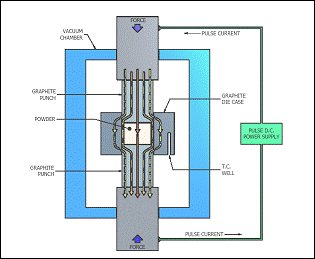
\includegraphics[width=0.4\textwidth]{../../Documentacion/Diagramas/image004.jpg}
  \end{center}
  \caption{SPS}
  \vspace{-20px}
  \end{wrapfigure}

  En el mercado encontramos soluciones de gran emplazamiento y envergadura, como lo son los propuestos por \href{''http://thermaltechnology.com/index.php?option=com_content&view=article&id=84''}{Thermal Technology LLC}
  basado en la tecnología de Spark Plasma Sintering (SPS) un revolucionario en polvo de alta velocidad de proceso de consolidación.
  SPS utiliza alto pulsos de alta corriente continua para activar la consolidación y la reacción de sinterización de los
  materiales. Un sistesma de SPS trabaja con materiales conductores, no conductores y compuesto a cualquier nivel de densidad.
  La ventaja de SPS es ahorro de tiempo y energía y la capacidad de retener nanoestructuras.


  %--------------------------------------------------------------------------------------------------------------------  
  %--------------------------------------------------------------------------------------------------------------------

  \subsubsection{Planes de crecimiento}  
  El proyecto en un principio propone realizar la automatización del proceso de sinterizado estableciendo las normas de seguidad
  que corresponden. En un segundo paso, realizar las medeciones sobre las mágnitudes involucradas en el proceso. Tensión, corriente
  tiempo de descarga, etc, y su posterior almacenamiento. Finalmente todo lo anterior se lo integraría de forma que pueda sincronizar
  contra un servidor en red.

  %--------------------------------------------------------------------------------------------------------------------  
  %--------------------------------------------------------------------------------------------------------------------

  \subsubsection{Objetivos de costo}  
  El objetivo propuesto trata de desarrollar instrumental de bajo o mediano costo en comparación a las opciones propuestas por
  la competencia. Desde ese punto de vista, el proceso de sinterizado a través de descarga de los capacitores propuesto es mas 
  eficiente

  %--------------------------------------------------------------------------------------------------------------------  
  %--------------------------------------------------------------------------------------------------------------------

  \newpage


%--------------------------------------------------------------------------------------------------------------------  
%--------------------------------------------------------------------------------------------------------------------

  \subsection{Factibilidad legal y responsabilidad civil (regulaciones y licencias}  

  \newpage


%--------------------------------------------------------------------------------------------------------------------  
%--------------------------------------------------------------------------------------------------------------------

  
  \newpage


%--------------------------------------------------------------------------------------------------------------------  
%--------------------------------------------------------------------------------------------------------------------

  \section{Ingeniería de detalle}  

    %\documentclass[12pt]{article}

%\usepackage{graphicx}
%\usepackage{caption}

%\begin{document}

%--------------------------------------------------------------------------------------------------------------------  
%--------------------------------------------------------------------------------------------------------------------

  \subsection{Hardware}  


%--------------------------------------------------------------------------------------------------------------------  
%--------------------------------------------------------------------------------------------------------------------

  \subsubsection{Detalles de selección y calculo de los elementos circuitales de cada bloque}  

  \newpage


%--------------------------------------------------------------------------------------------------------------------  
%--------------------------------------------------------------------------------------------------------------------

  \subsubsection{Plan de pruebas de cada modulo}  

  \newpage


%--------------------------------------------------------------------------------------------------------------------  
%--------------------------------------------------------------------------------------------------------------------

  \subsection{Software}  

  \newpage


%--------------------------------------------------------------------------------------------------------------------  
%--------------------------------------------------------------------------------------------------------------------

  \subsubsection{Diagrama de estados, procesos y flujogramas}  

  \newpage



%--------------------------------------------------------------------------------------------------------------------  
%--------------------------------------------------------------------------------------------------------------------

  \subsubsection{Análisis de complejidad (Mc.Cabe o Hasltead )}  

  \newpage



%--------------------------------------------------------------------------------------------------------------------  
%--------------------------------------------------------------------------------------------------------------------

  \subsubsection{Descripción de subrutinas}  

  \newpage



%--------------------------------------------------------------------------------------------------------------------  
%--------------------------------------------------------------------------------------------------------------------

  \subsubsection{Listados comentados del código }  

  \newpage


%--------------------------------------------------------------------------------------------------------------------  
%--------------------------------------------------------------------------------------------------------------------

  \subsubsection{Plan de prueba de módulos y de depuración de software}  

  \newpage

%--------------------------------------------------------------------------------------------------------------------  
%--------------------------------------------------------------------------------------------------------------------
%\end{document}


  \newpage

%--------------------------------------------------------------------------------------------------------------------  
%--------------------------------------------------------------------------------------------------------------------

  \section{Construcción del prototipo}  

    
%--------------------------------------------------------------------------------------------------------------------  
%--------------------------------------------------------------------------------------------------------------------

  \subsection{Definición de los módulos}  

  \newpage


%--------------------------------------------------------------------------------------------------------------------  
%--------------------------------------------------------------------------------------------------------------------

  \subsection{Diseño de los circuitos impresos}  

  \newpage



%--------------------------------------------------------------------------------------------------------------------  
%--------------------------------------------------------------------------------------------------------------------

  \subsection{Diseño mecánico}  

  \newpage

%--------------------------------------------------------------------------------------------------------------------  
%--------------------------------------------------------------------------------------------------------------------

%--------------------------------------------------------------------------------------------------------------------  
%--------------------------------------------------------------------------------------------------------------------

  \subsection{Detalles de construcción y precauciones especiales de montaje}  

  \newpage



%--------------------------------------------------------------------------------------------------------------------  
%--------------------------------------------------------------------------------------------------------------------


  \newpage

%--------------------------------------------------------------------------------------------------------------------  
%--------------------------------------------------------------------------------------------------------------------
% 
  \section{Validación del prototipo}  

    


%--------------------------------------------------------------------------------------------------------------------  
%--------------------------------------------------------------------------------------------------------------------

  \subsection{Validación de hardware}  

  \newpage



%--------------------------------------------------------------------------------------------------------------------  
%--------------------------------------------------------------------------------------------------------------------

  \subsubsection{Plan y protocolos especiales de medición}  

  \newpage




%--------------------------------------------------------------------------------------------------------------------  
%--------------------------------------------------------------------------------------------------------------------

  \subsubsection{Medidas}  

  \newpage



%--------------------------------------------------------------------------------------------------------------------  
%--------------------------------------------------------------------------------------------------------------------

  \subsubsection{Evaluación}  

  \newpage




%--------------------------------------------------------------------------------------------------------------------  
%--------------------------------------------------------------------------------------------------------------------

  \subsubsection{Resultados}  

  \newpage




%--------------------------------------------------------------------------------------------------------------------  
%--------------------------------------------------------------------------------------------------------------------

  \subsection{Validación de software}  

  \newpage

%--------------------------------------------------------------------------------------------------------------------  
%--------------------------------------------------------------------------------------------------------------------


  \newpage

%--------------------------------------------------------------------------------------------------------------------  
%--------------------------------------------------------------------------------------------------------------------

  \section{Estudios de confiabilidad de hardware y de software}  
  
  %------------------------------------------------------------

\section{Estudios de confiabilidad de hardware y software }


  
  \newpage


%--------------------------------------------------------------------------------------------------------------------  
%--------------------------------------------------------------------------------------------------------------------

  \section{Conclusiones}  

    %--------------------------------------------------------------------------------------------------------------------  
%--------------------------------------------------------------------------------------------------------------------

  \subsection{Excelencias. Objetivos alcanzados}  

  \newpage


%--------------------------------------------------------------------------------------------------------------------  
%--------------------------------------------------------------------------------------------------------------------

  \subsection{Fallos. Recomendaciones para futuros diseños}  

  \newpage


%--------------------------------------------------------------------------------------------------------------------  
%--------------------------------------------------------------------------------------------------------------------


  \newpage


%--------------------------------------------------------------------------------------------------------------------  
%--------------------------------------------------------------------------------------------------------------------

  \section{Anexos: Técnicos. Justificativos. Descriptivos. Documentales}  

    
  \subsection{Planos}  

  \newpage



%--------------------------------------------------------------------------------------------------------------------  
%--------------------------------------------------------------------------------------------------------------------

  \subsection{Esquemas}  

  \newpage


%--------------------------------------------------------------------------------------------------------------------  
%--------------------------------------------------------------------------------------------------------------------

  \subsection{Listado de partes}  

  \newpage



%--------------------------------------------------------------------------------------------------------------------  
%--------------------------------------------------------------------------------------------------------------------

  \subsection{Códigos de software}  

  \newpage



%--------------------------------------------------------------------------------------------------------------------  
%--------------------------------------------------------------------------------------------------------------------

  \subsection{Experiencias accesorias}  

  \newpage



%--------------------------------------------------------------------------------------------------------------------  
%--------------------------------------------------------------------------------------------------------------------

  \subsection{Hojas de datos de componentes}  

  \newpage



%--------------------------------------------------------------------------------------------------------------------  
%--------------------------------------------------------------------------------------------------------------------

  \subsection{Hojas de aplicación, etc.}  

  \newpage



%--------------------------------------------------------------------------------------------------------------------  
%--------------------------------------------------------------------------------------------------------------------

  \subsection{Manuales de operación, soporte e instalación}  

  \newpage

%--------------------------------------------------------------------------------------------------------------------  
%--------------------------------------------------------------------------------------------------------------------

  \newpage

%--------------------------------------------------------------------------------------------------------------------  
%--------------------------------------------------------------------------------------------------------------------



  %Bibliografia


% Bibliografía 
%  LIBROS.- Autor. Título. Editorial. Fecha 
%  REVISTAS.- Autor. Título. Nombre de la revista. FechaVolumen. Páginas, Notas de aplicación (incluir copia de las importantes)

  \newpage

  \begin{thebibliography}{1}
    \bibitem{} 

  \end{thebibliography}
    

\end{document}
